%Лекция 1
\paragraph*{}\note{Традиционно, деление живых организмов на царства осуществляется на основе особенностей организации их клетки. Ниже приведены особенности строения клетки растений, которые служат основанием для выделения растений в отдельное царство Planta.}

\paragraph*{}Клетка — основная функциональная часть растительного организма. 
%У растений, в отличии от животных нет систем органов. 

\paragraph*{}Все растения являются многоклеточными организмами, клетки которых дифференцированы согласно выполняемым функциям \footnote{В 70-80 годах растения разделяли на высшие и низшие. В последнюю группу включались ряд одноклеточных организмов, таких как хлорелла и хламидомонада. Однако сейчас все одноклеточные организмы объеденные в царство Простейшие}

\paragraph*{}Строение растительной клетки во многом сходно со сторением клеток животных и грибов: как и у всех \hyperlink{q_prok_cell}{\termin{эукариотических}} организмов, клетки растений имеют в своем составе ядро, цитоплазму, ряд клеточных органелл и систему мембран (\ris \ref{cell_shema}) \footnote{Так как строение клетки и функции ее компонентов подробно рассматриваются на курсе <<Цитология>>, то мы не будем подробно останавливаться на общих чертах растительной клетки а опишем лишь структуры характерные только для клеток растений. Общее же строение клетки можно повторить на основе учебника по физиологии растений, например В.М. Юрина \cite{urin_2010}.}

\paragraph*{}Специфической особенностью строения растительной клетки является:

\begin{enumerate}
    \item наличие прочной полисахаридной \hyperlink{cell_wall}{клеточной стенки}
    \item наличие крупной \hyperlink{cell_vakuol}{центральной вакуоли}
	\item наличие системы \hyperlink{cell_plastids}{пластид}
	
\end{enumerate}

%%%%%%%%%%%%%%%%%%%%%%%%%%%%%%%%%%%%%%%%%%%%%%%%%%%%%%%%%%%%%%%%%%%%%%%%%%%%%%%%%%%%%%%%%%%%%%%%%%%%%%%%%%% 
\begin{figure}
  \centering
       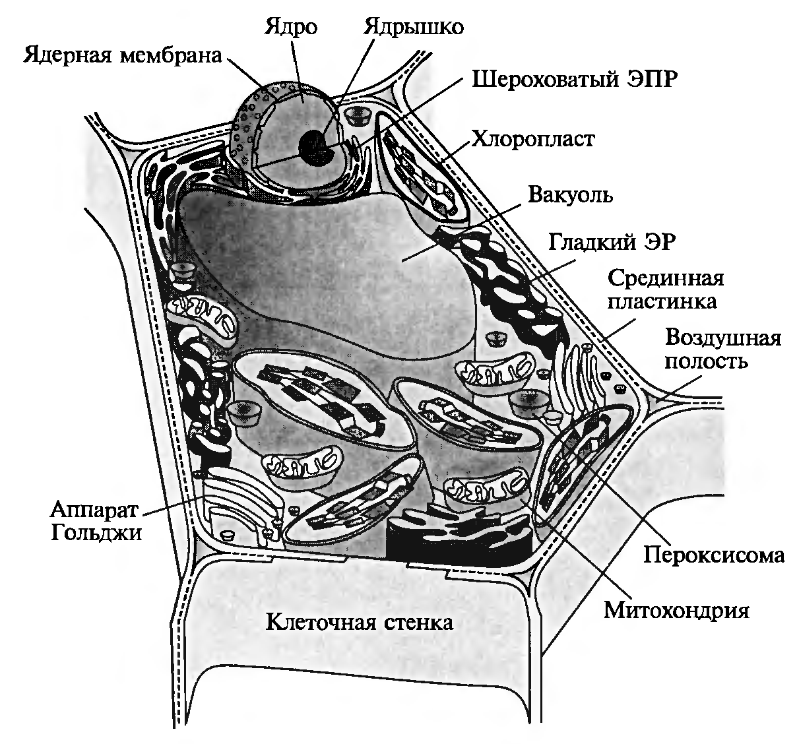
\includegraphics[width=0.5\linewidth]{pictures/plant_cell}
\caption{Строение растительной клетки}
\label{cell_shema}
\end{figure}
%%%%%%%%%%%%%%%%%%%%%%%%%%%%%%%%%%%%%%%%%%%%%%%%%%%%%%%%%%%%%%%%%%%%%%%%%%%%%%%%%%%%%%%%%%%%%%%%%%%%%%%

%\paragraph*{}Растительная клетка содержит три относительно автономные, но тесно взаимодействующие генетические системы: 1. ядерную, 2. митохондриальную и 3. пластидную. Для растительных клеток характерен особый тип роста – рост растяжением. У делящихся растительных клеток отсутствуют центриоли. Клеточные стенки всех клеток контактируют друг с другом, образуя единую систему стенок — апопласт. 

\subsection*{Клеточная стенка}

\paragraph*{}Химический состав и структура \hypertarget{cell_wall}{клеточной стенки} обеспечивают ее важнейшие свойства -- прочность, эластичность и высокую способность впитывать воду -- \termin{гидрофильность}.

\paragraph*{}Основой химического состава клеточной стенки являются полисахариды: \hyperlink{cellulosa}{целлюлоза} -- 25\%, гемицеллюлоза -- 40 \% и пектиновые вещества -- 30 \%. На долю белков и остальных веществ приходится только 5 \% от массы клеточной стенки. 

\paragraph*{}Тонкие нити целлюлозы переплетаются образуя сеть, которая погружена в аморфный \termin{матрикс}.

\paragraph*{}\note{Таким образом, клеточная стенка напоминает по структуре железобетон, где сеть из железных прутьев погружена в слой бетона}

\paragraph*{}В клеточной стенке различают первичную и вторичную оболочки.

\paragraph*{}Первичная оболочка отличается большим количеством гемицеллюлозы и пектина. Она очень гигроскопична. Формирование первичной оболочки заканчивается с окончанием роста клетки.

\paragraph*{}Вторичная оболочка начинает формироваться по окончании роста клетки. Откладывается на внутренней поверхности клеточной стенки. Образованна целлюлозой.

\paragraph*{}Между первичными оболочками соседних клеток находится прослойка пектина -- \termin{серединная пластинка}. При разрушении срединной пластинки (\termin{мацерации}) клетки разъединяются.

\paragraph{Функции клеточной стенки}

\begin{enumerate}

	\item Опорная-- КС придает постоянную форму растительным клеткам, и растения в целом \footnote{На прочности клеточной стенки основано функционирование механических тканей растения - колленхимы и склеренхимы}
	\item Защитная -- КС защищает клетку от разрушения гидростатическим давлением и от проникновения инфекций.
	\item Принимает участие в поглощении минеральных веществ.

\end{enumerate}

\paragraph*{}Клеточная стенка пронизана порами \termin{\hypertarget{plasmodesma}{плазмодесмами}}, благодаря которым цитоплазма всех клеток объединена в единое целое -- \termin{симпласт}. Через плазмодесмы осуществляется транспорт воды, минеральных веществ и гормонов.


\paragraph*{}Каждая плазмодесма представляет собой тяж \termin{гиалоплазмы}, окруженный плазмалеммой, центральную часть которого занимает \termin{десмотрубка}, которая связывает эндоплазматический ретикулум соседних клеток. Непрерывную систему эндоплазматического ретикулума растения называют эндопластом.

%\paragraph*{}Клеточная стенка. Состоит из целлюлозы, гемицелюлозы и пектиновых веществ, липиды и небольшое количество белков. В стареющих клетках оболочки пропитываются лигнином и суберином. Кроме того, в оболочках растительных клеток найдены ферменты.

\subsection*{Цитоплазматическая мембрана и протопласт}

\paragraph*{}\hypertarget{plasmolema}{Клеточная мембрана} или \termin{плазмолема}, находится под клеточной стенкой. Основу мембраны составляет двойной слой \hyperlink{plipids}{фосфолипидов}. Важной составляющей частью плазмолемы являются так же белки и гликолипиды. 

\paragraph*{}Белки, входящие в состав цитоплазматической мембраны делятся на две группы

\begin{enumerate}
	\item Переферийные белки -- гидрофильные белки, которые возможно легко отделить от мембраны
	\item Интегральные -- гидрофобные белки, прочно связанные с мембраной \cite{fzr_ermakov}
\end{enumerate}

\paragraph*{}Функции мембранных белков

\begin{enumerate}

	\item \hyperlink{enzimes}{ферменты} катализируют ассоциированные с мембраной реакции. 
	\item структурные белки, не имеют ферментативной активности, образуют мембраны
	\item транспортные белки, переносят вещества через мембраны,
	\item белки-рецепторы, воспринимают раздражения,
	\item обеспечивают связь плазмалеммы с цитоскелетом.

\end{enumerate}

\paragraph{Функции плазмолемы}

\begin{enumerate}
	\item Транспортная -- избирательно пропускает вещества из и внутрь клетки.
	\item Осмотическая -- поддерживает осмотические свойства клетки.
	\item Регуляторная -- регулируют обмен веществ (транспорт веществ, активность ферментов);
	\item Структурная -- делят клетку на компартменты (замкнутые полости), имеющие разный химический состав; благодаря мембранам в клетке возникают разные градиенты (химического состава, концентрации, электрические, вязкости);
\end{enumerate}

\remember{\textbf{Избирательная проницаемость} -- это ключевое свойство всех биологических мембран, лежащие в основе способности клетки к поддержанию постоянства состава внутренней среды}

\paragraph*{}\hypertarget{protoplast}{Протопласт} -- живое содержимое клетки. Протопласт состоит из \hypertarget{citoplasma}{цитоплазмы} и органелл: ядра, митохондрий, аппарата Гольджи, рибосом и др., погруженных в матрикс цитоплазмы — гиалоплазму.

\paragraph*{}По химическому составу цитоплазма на 80\% состоит из воды, а на 20\% из сухого вещества -- белков и небольшого количества липидов.

\paragraph*{}Ядро: основная органелла клетки, где сосредоточена большая часть наследственной информации. В молодой клетки -- в центре, потом смещается центральной вакуолью на периферию клетки. Оболочка ядра двойная с порами. Цитоплазма ядра \termin{кариоплазма} содержит деспирализованые хромосомы -- \termin{хроматин}, одно или несколько ядрышек.

\paragraph*{}Функция ядра -- хранение и передача наследственной информации.

\paragraph*{}\hypertarget{mitohondria}{Митохондрии} -- тела палочковидной формы, число митохондрий зависит от физиологического состояния клетки (десятки или тысячи). Имеют сложную структуру: двойная мембрана образует впячивания кристы, на поверхности которых ферменты дыхательной цепи.

\paragraph*{}\note{В отличии от клеток животных, содержащих, как правило, одну большую разветвленную митохондрию, клетки растений содержать множество мелких митохондрий}%Надо проверить и указать литературу

\paragraph*{}Функция митохондрий — участие в аэробном этапе дыхания.

\paragraph*{}\hypertarget{sect_rybosoms}{Рибосомы} -- немембранные органелы, которые состоят из двух субъединиц (большей и малой) и представляют собой сложный комплекс из \hyperlink{proteins}{белков} и \gls{rna}. Функция рибосом -- участие в синтезе белка на этапе трансляции.

\paragraph*{}Комплекс Гольджи представляет собой стопу одномембранных цистерн -- \termin{диктиосом}. Количество таких цистерн может быть различно в зависимости от типа и стадии развития клетки.

\paragraph*{}\note{Например в клетках апикальной меристемы иван-чая содержится примерно 20 единиц, а в клетках хлопка, которые продуцируют волокна -- более 1000 \cite{fzr_ermakov}.} 

\paragraph*{}В отличии от животной клетки, где КГ локализован в центре клетки, в растительной клетки диктиосомы комплекса Гольжджи рассеяны по всей цитоплазме. Кроме того КГ в клетки растения остается целостным и активным в течении \termin{\hyperlink{q_mitos}{митоза}}, чтобы обеспечить синтез клеточной стенки  \cite{fzr_ermakov}.

\paragraph*{}Эндоплазматический ретикулум — система каналов образованных одной мембраной, пронизывающих цитоплазму, связанных с ядром и ретикулумом других клеток через плазмодемсмы. Функции -- участие в синтезе белка, транспорт веществ, разделение клетки на отсеки

\subsection*{Центральная вакуоль}

\paragraph*{}\hypertarget{cell_vakuol}{Центральная вакуоль} это одномембранная органелла характерна только для растительных клеток. Мембрана центральной вакуоли носит название \gls{tonoplast}. В ходе \hyperlink{ontogenesis}{онтогенеза} растительной клетки центральная вакуоль формируется из мелких протовакуолей. У зрелой клетки центральная вакуоль занимает большую часть объема.

\paragraph*{}Функции центральной вакуоли 

\begin{enumerate}
	\item Увеличение площади поверхности клетки \note{Для растений, как для фототрофных организмов, важна большая площадь поверхности клеток, позволяющая разместить большее количество хлоропластов. Центральная вакуоль позволяет увеличить размер, а следовательно и площадь поверхности клетки не за счет структурированной богатой азотом цитоплазмы, а за счет большей вакуоли, наполненной <<дешевым для производство>> соком \cite{fzr_ermakov}}
	\item Создание и поддержание тургорного давления
	\item Регуляция pH --вакуоль служит резервуаром для протонов
	\item Защитная --в вакуоли содержится ряд веществ, защищающих растения от поедания насекомыми и млекопитающими. Среди данных веществ можно выделить токсины (фенольные соединения, алкалоиды), полимеры (каучук, гутта), ферменты
	\item Участие в придании растению окраски -- вакуоли могут содержать водорастворимые пигменты (антоцианы и беталаины) 
	\item Запасание питательных веществ
	\item Запасание вредных для клетки веществ -- внутри вакуолей растения утилизируют токсины и тяжелые металлы в виде оксалатов (\ris \ref{crystals}) и избавляются от них в результате листопада.
\end{enumerate}

%%%%%%%%%%%%%%%%%%%%%%%%%%%%%%%%%%%%%%%%%%%%%%%%%%%%%%%%%%%%%%%%%%%%%%%%%%%%%%%%%%%%%%%%%%%%%%%%%%%%%%%%%%% 
\begin{figure}
  \centering
       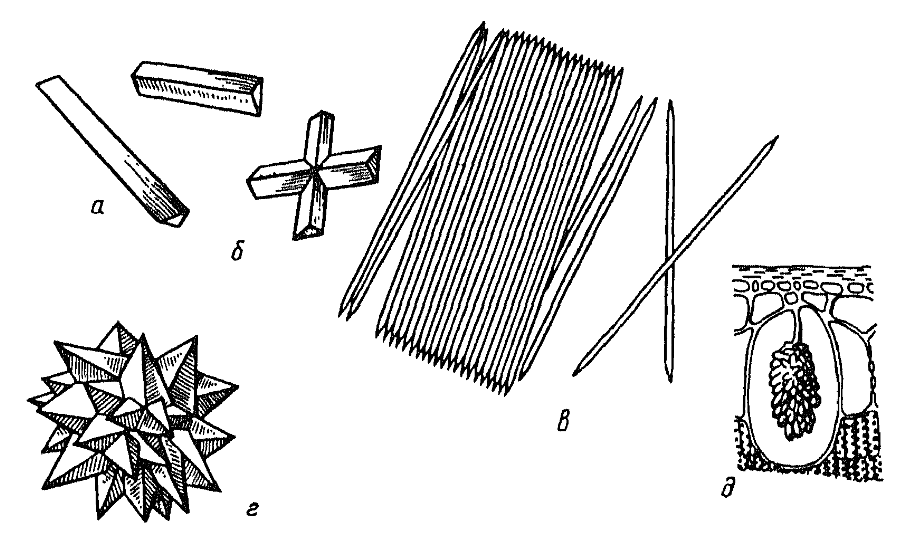
\includegraphics[width=0.5\linewidth]{pictures/crystals}
\caption{Различные типы включений из вакуолей растительной клетки (согласна И.И. Андреевой \cite{andreeva-bot})}
\label{crystals}
\end{figure}
%%%%%%%%%%%%%%%%%%%%%%%%%%%%%%%%%%%%%%%%%%%%%%%%%%%%%%%%%%%%%%%%%%%%%%%%%%%%%%%%%%%%%%%%%% 

\subsection*{Пластиды}

\paragraph*{}\hypertarget{cell_plastids}{Пластиды} делятся на: 

\begin{enumerate}

	\item Хлоропласты 
	\item Хоромопласты 
	\item Лейкопласты (\ris \ref{plastids}). 
	\item Этиопласты

\end{enumerate}



%%%%%%%%%%%%%%%%%%%%%%%%%%%%%%%%%%%%%%%%%%%%%%%%%%%%%%%%%%%%%%%%%%%%%%%%%%%%%%%%%%%%%%%%%%%%%%%%%%%%%%%%%%% 
\begin{figure}
  \centering
       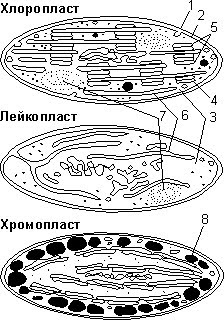
\includegraphics[width=0.3\linewidth]{pictures/plastids}
\caption{Различные типы пластид}
\label{plastids}
\end{figure}
%%%%%%%%%%%%%%%%%%%%%%%%%%%%%%%%%%%%%%%%%%%%%%%%%%%%%%%%%%%%%%%%%%%%%%%%%%%%%%%%%%%%%%%%%% 

\subsubsection*{Хлоропласты}

\paragraph*{}\hyperlink{question_hloroplast}{Хлоропласты} -- двумембранные органоиды линзообразной формы и размером 4-10 мкм. Внутренняя мембрана хлоропласта образует многочисленные впячивания -- \termin{тилакоиды}, служащие для увеличения ее поверхности. Стопка, образованная внутренними мембранами -- тилакоидами называется \termin{грана}. Соседние граны связаны одиночными мембранами-тилакоидами, носящими название \termin{ламеллы}. На мембранах тилакоидов находятся пигменты (хлорофиллы) и белки, принимающие участие в фотосинтеза.

\paragraph*{}Внутри хлоропласта есть своя цитоплазма -- \termin{матрикс}, свои рибосомы. Хлоропласты имеют кольцевую ДНК и все необходимые для синтеза \hyperlink{proteins}{белка} компоненты. Геном хлоропластов кодирует лишь часть необходимых белков; другую часть кодирует ядерный геном фотосинтезирующей клетки. 

\paragraph*{}Хлоропласты возникают \textit{de novo} из инициальных частиц, а также могут размножаться путем простого деления.

\paragraph*{}В растениях хлоропласты локализуются в основном клетках листьев и молодых стеблей. Число хлоропластов обычно составляет от 20 до 100 на клетку. Хлоропласты содержат следующие типы пигментов:

\begin{enumerate}

\item хлорофиллы А и B
\item каротиноиды (оранжевый каротин и желтый ксантофилл)

\end{enumerate}

\paragraph*{}Основная функция хлоропластов -- фотосинтез \footnote{Более подробно строение и функции хлоропластов будут рассмотрены в разделе, посвященном фотосинтезу}. Хлоропласты большинства растений способны перемещаться по клетке в зависимости от интенсивности и направления освещения.

\subsubsection*{Остальные пластиды}

\paragraph*{}Хромопласты встречают в клетках лепестков, зрелых плодов, листьев.
Форма хромопластов может быть: 

\begin{enumerate}

	\item дисковидная
	\item шаровидная
	\item палочковидная
	\item веретенообразная

\end{enumerate}

\paragraph*{}Хромопласты содержат красные, оранжевые и желтые пигменты из группы каротиноидов. Функция хромопластов -- привлечение насекомых-опылителей и животных-распространителей семян.

\paragraph*{}Лейкопласты – бесцветные пластиды, шарообразной или веретенообразной формы. 

\paragraph*{}Функция лейкопластов -- запас питательных веществ. 

\note{Особенно много лейкопластов в запасающих органах – корнях, семенах, плодах, молодых листьях и др.}

\paragraph*{}В зависимости от природы накапливающихся веществ лейкопласты делят на:

\begin{enumerate}

	\item амилопласты -- запасаются углеводы (в большинстве случаев)
	\item олеопласты -- запасаются жиры 
	\item протеинопласты -- запасаются белки

\end{enumerate}

\paragraph*{}этиопласты -- пластиды, формирующиеся при недостаточном освещении и не содержащие хлорофиллов

\subsection*{Вопросы и задания для самоконтроля}

\begin{enumerate}
	\item{Повторите строение \hypertarget{q_prok_cell}{прокариотической клетки}. Составьте таблицу, отражающую различия в строении прокариотической и эукариотической клеток.}
	\item На какие стадии подразделяется \hypertarget{q_mitos}{митоз}, чем деление путем митоза отличается от мейотического деления? Данные сведения вы можете повторить по любому учебнику общей биологии.
	\item Сравните строение \hypertarget{question_hloroplast}{хлоропласта} и бактериальной клетки. В чем проявляется сходство между ними, а в чем различия.
\end{enumerate}


